\section{Literature Survey}	

In many midsurface generation approaches, simplification/defeaturing and cellular decomposition is used for pre-processing.  Following sub-sections evaluate some of the relevant past works in these domains.
 
 \subsection{Midsurface Generation Approaches}
 
Midsurface is a special case of a more generic structure called ``Medial Object''. Medial Object is the geometry that is midway inside an input shape. The input shape can be an image, a 2D profile or a 3D solid. One of the early works in the field of Medial object was by a theoretical biologist, Harry Blum in 1967 \cite{Harry1967}. Following are some of the salient approaches  (Figure \ref{fig:medials}) :

\bigskip

	\begin{figure} [!h]
		\centering
		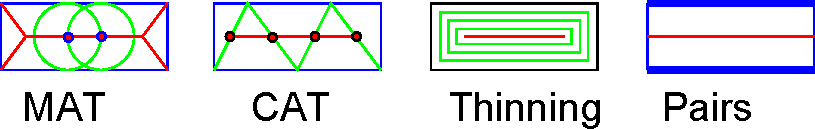
\includegraphics[width=0.7\linewidth]{..//Common/images/MedialMethodsOnlyShort.pdf}
		\caption{Medial Generation Approaches}
		\label{fig:medials}
	\end{figure}


\begin{itemize}[noitemsep,topsep=2pt,parsep=2pt,partopsep=2pt]%leftmargin=*
	\item  \textbf{Medial Axis Transform (MAT)}: MAT is a locus of the center of an inscribed maximal disc as it rolls around the object's interior. It can be generated for any shape. The major drawback of this approach is that it creates unnecessary branches and gives unpredictable output upon perturbations in the input shape \cite{Attali2004}.
	\item \textbf{Chordal Axis Transform (CAT)}: The input shape is constrained-triangulated and chord midpoints are joined to form the medial \cite{QuadrosRoshanOwenBrewerShimada2004}. Drawback of CAT is that quality of medial heavily depends on the triangulation, which in turn, can be error-prone.
	\item \textbf{Thinning}: Medial is generated similar to the grass-fire process by successively offsetting its boundary toward its interior until vanishing \cite{Montanari1969}. Drawback of Thinning is that it generates branches which need to be post-processed to arrive at a midcurve.
	\item \textbf{Midsurface Abstraction (MA), Face Pairing}: MA, initiated by Rezayat \cite{Rezayat1996},  involves identifying ``face pairs'' in the final solid shape, generating midsurface patches for each face-pair and then building a connected midsurface by extending or trimming and then joining the patches. Major problems are faced in the identification of the face-pairs as well as in joining the midsurface patches. Manual/semi-automatic patching method have to be provided to correct the failures.
\end{itemize}

\subsection{Model Simplification Approaches}
 
Model Simplification/Defeaturing involves removal of features irrelevant to the application-context. Thakur et al. \cite{Thakur2009} surveyed and classified various approaches used till then, into categories such as surface-based, volume-based and feature-based.  

Dabke \cite{Dabke1994} through the concept of ``global idealization'', was one of the first researchers to leverage the feature information for defeaturing. Lee \cite{SangHunLee2005} elaborated an approach to reorder features in the history tree and then build partly up to a given level of simplification. Russ \cite{Russ2012} decided suppressibility on the feature type, feature dimensions, proximity of features to the boundary conditions, analysis type and part dimensions. Commercial packages like Autodesk Fusion\textsuperscript{\textregistered}, Altair's Hypermesh\textsuperscript{\textregistered},  etc. also provide similar defeaturing capabilities mainly for CAE analysis, but have to do heuristic feature recognition first, which is prone to failures. 
  
 \subsection{Cellular Decomposition}
 
Cellular decomposition, in the context of the current research, is the division of a feature-based CAD model into volumetrically adjacent bodies called ``cells''.  Research in  cellular decomposition, especially for Computer-aided Manufacturing (CAM) and CAE has been going on for decades. Feature-based cellular decomposition, which deals with either decomposition of features, or feature-recognition after decomposition,  has also been  researched extensively \cite{Bidarra1993,Woo2003, Boussuge2013}. There have been a few attempts to generate a midsurface using cellular-decomposition as well \cite{Chong2004, Woo2013, Boussuge2013, Zhu2015}, but the methodologies presented therein appear to be limited due to extensive use of heuristic rules such as hard-coded values for detecting edge/face pairs, support for limited types of geometries, only limited scope in terms of the range of connections  handled, etc. For example, Woo's \cite{Woo2013} approach, uses face-pairing using distance criteria, which may generate incorrect pairs. It is restricted to only analytical surfaces and only parallel face-pairs.% The proposed research tries to overcome many of these limitations.

\subsection{Observations of Literature Survey} \label{sec:litsurvey:analysis}
 
After analyzing various past approaches, both in the academic and commercial domains, it was concluded that there has been limited success in the generation of a well-connected midsurface. 
Some of the salient observations are:
 
\begin{itemize}[noitemsep,topsep=2pt,parsep=2pt,partopsep=2pt]%leftmargin=*

	\item  In feature-based model-simplification approaches, full feature dimensions are used for selecting the candidates for removal \cite{Russ2012} thereby giving wrong results, as in most cases, the feature volume is consumed in the final model, which should ideally be ignored.
	\item Domain-specific rules of identification of candidate features for removal is necessary instead of plain size based selections \cite{AdskElectronicsHelp}.
	\item Past midsurface generation approaches are limited in the range of geometries (say, only planar or analytic surfaces), feature types (say, only extruded, positive primitives) and connection types (say, only, parallel, or perpendicular) they could handle \cite{Woo2013}. 
	\item  %\textbf{Midsurface Patches Generation}:  \label{sec:facepairdetection}
In face pairing approaches, finding the face-pairs in a complex part itself is very challenging \cite{Boussuge2013}. In non-trival models, issues like faces may not be directly opposite to each other, may not be parallel, may have multiple candidates, etc. arise resulting in gaps in the midsurface. %This research addresses this problem by using the Abstracted feature-information for generation of patches and avoids detection of face-pairs  (more details in section \ref{sec:scell}). 
	\item  %\textbf{Midsurface Patches Connection}: \label{sec:facepairinteraction}
There is no theoretical framework encompassing all the possible connection types, providing a unified logic to join midsurface patches has not been possible \cite{Stolt2006}. %This research proposes  leveraging of feature-based cellular decomposition (more details in section \ref{sec:icell}).
\end{itemize}
 
 %The proposed approach is `generic', meaning, in principle, no such restrictions are present in this approach. It can be made to cater to any geometry types, feature types or connections. Advantages can be seen in the range of shapes handled as well as in the minimization of failures (Section \ref{sec:results}).
 
 
 \subsection{Research Scope}
The proposed research aims at developing algorithms for generating well-connected midsurface of thin-walled parts. Domain selected is of sheet metal parts. Sheet metal models are unique in both, geometrical and topological sense. They are characterized by:
\begin{itemize}[noitemsep,topsep=2pt,parsep=2pt,partopsep=2pt]
\item \textbf{Constant thickness}: Made up of constant thickness blank roll.
\item \textbf{Absences}: There are no blind holes, but only through holes, if any. 
\item \textbf{Degeneracy}: There are no degenerate capping thickness faces (like ``Wedge'').
\item \textbf{Cavities}: There are no embedded volumes or cavities (``bubbles'').
\end{itemize}

%Geometrical and topological characteristics of Sheet metal models are:
%\begin{itemize}[noitemsep,topsep=2pt,parsep=2pt,partopsep=2pt]
%\item \textbf{Constant thickness}: Made up of constant thickness blank roll.
%\item \textbf{Absences}: There are no blind holes, but only through holes, if any. 
%\item \textbf{Degeneracy}: There are no degenerate capping thickness faces (like ``Wedge'').
%\item \textbf{Cavities}: There are no embedded volumes or cavities (``bubbles'').
%\end{itemize}

CAD models of sheet metal parts use a wide variety of feature such as \cite{Liu2004}:

\begin{minipage}[c]{0.98\linewidth}
\begin{minipage}[t]{0.48\linewidth}
\begin{itemize}[noitemsep,topsep=2pt,parsep=2pt,partopsep=2pt]
\item \textbf{Primitive features}: These features an exist interdependently and form primary shape of the part, e.g. Wall, Drawing.
\item \textbf{Add-on features}: These features must be added to the existing features and are secondary in nature, e.g. Cutout, Hole, Slot.
\item \textbf{Connecting features}: These features act as a bridge between other features, e.g. Bend.
\item \textbf{Composite features}: These are feature collections, .e.g. Array.
\end{itemize}
\end{minipage}
\hfill
\begin{minipage}[t]{0.48\linewidth}
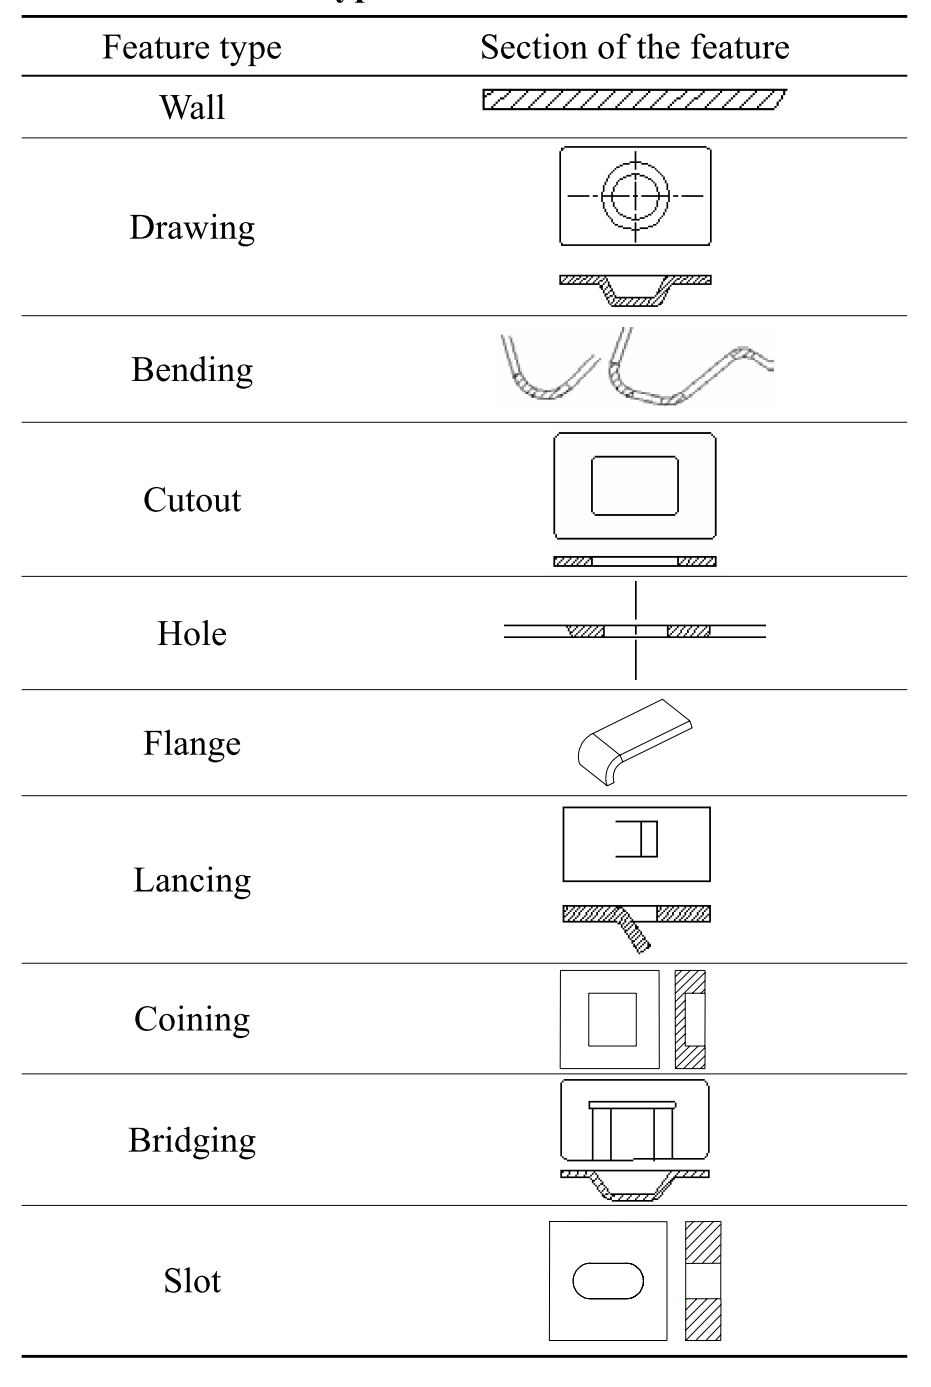
\includegraphics[width=0.52\linewidth,valign=t]{..//Common/images/liuFeatures}
\captionof{figure}{Typical Sheet metal features \cite{Liu2004}}\label{fig:liufeatures}
\end{minipage}
\end{minipage}

The proposed system works on the sheet metal feature-based CAD models as input, having features similar to ones mentioned above. In particular, it caters to parts made by fabrication, which show significant problems in generating midsurface, especially at the joints. Iit should be possible to extend it to variable-thickness components as well, with further customizations. 

\subsection{Research Objectives} \label{sec:litsurvey:rquestions}

The primary objective of the proposed research is to develop a system to generate a well-connected midsurface of sheet metal feature-based CAD model. This objective is broken down further into following sub-objectives:
\begin{itemize}[noitemsep,topsep=2pt,parsep=2pt,partopsep=2pt]
\item To develop and implement a feature-based model simplification (defeaturing) approach to generate a ``gross shape'', which improves midsurface generation.
\item To develop and implement a feature abstraction approach to further simplify the model, by transforming each feature to a generalized form, reducing the number of scenarios to handle.
\item To develop and implement a generic midsurface generation approach leveraging generalized feature form and cellular decomposition.
\item To develop a topological validation methodology to assess correctness of the midsurface.
\item To test real-life parts to demonstrate efficacy of the proposed approach.
\end{itemize}

Following section elaborates how the proposed system aims at satisfying these objectives.

%T
%
%\begin{myhyp}
%\label{hyp:features}
%Instead of working on the final shape (Brep), access to the feature information, in the form of tree/sequence will enable generation of deterministic midsurface via modules such as feature-based Simplification, feature-based-Abstraction, feature-based-Decomposition and feature-based-Midsurface generation.
%\end{myhyp}
%
%\begin{myhyp}
%\label{hyp:Simplification}
%Instead of working on the detailed CAD model, the simplified ``gross-shape'' results in more representative midsurface.
%\end{myhyp}
%
%\begin{myhyp}
%\label{hyp:Abstraction}
%Instead of working on plethora of features, the generalized Loft based representation will help devise a generic midsurface patch generation algorithm, thus addressing the complex face pairing problems.
%\end{myhyp}
%
%\begin{myhyp}
%\label{hyp:Decomposition}
%Instead of working on the full shape, the decomposition of the shape into primitive sub shapes, help address various connectivity issues and make the algorithm more generic? If the shape is decomposed into sub-shapes then piecewise transformation definition is possible, leading to an overall, formal representation for the midcurve/midsurface.
%\end{myhyp}
%
%\begin{myhyp}
%\label{hyp:MidsurfaceGeneration}
%The transformation of decomposed solid sub-shapes, with owner features, in the abstracted form, will result in a representative, well connected midsurface.
%\end{myhyp}
%
